% This is an example of how to use the "npsthesis" document style for theses
% Modified for personal use by Fabrice Ardhuin, 2001/03/10
%
%  TO DO : add http://upload.wikimedia.org/wikipedia/commons/d/db/Munk_ICCE_1950_Fig1.svg  in ch1 

\documentclass[a4paper]{book}  % psfig for Encapsulated PostScript
%\usepackage{fullpage}
\addtolength{\oddsidemargin}{-0.4in} \addtolength{\evensidemargin}{-1.1in}
\addtolength{\textwidth}{1.5in} \addtolength{\topmargin}{-0.5in}
\addtolength{\textheight}{1.4in}
\usepackage[pdftex]{graphicx}
\usepackage{amsmath}
\usepackage{bm}
\pdfcompresslevel9
\usepackage[american]{babel}
% %\usepackage{upmath}
\usepackage[latin1]{inputenc}
%\usepackage[pdflatex]{graphics}
\usepackage{makeidx}
\usepackage{hyperref}
\usepackage{float}
\usepackage[section]{placeins}
 \usepackage{xcolor}
\hypersetup{
    colorlinks,
    linkcolor={red!50!black},
    citecolor={blue!50!black},
    urlcolor={blue!80!black}
}

%\usepackage[pdftex,plainpages=false]{hyperref}
\usepackage{natbib}
\setlength{\bibsep}{0em}

%\degree{Doctor of Philosophy In Oceanography}

% these macros save typing:
\newcommand{\beq}{\begin{equation}}
\newcommand{\beqa}{\begin{eqnarray}}
\newcommand{\eeq}{\end{equation}}
\newcommand{\eeqa}{\end{eqnarray}}
%
%\newcommand\p3{Part 3}
%\newcommand\p2{Part 2}
%\newcommand\p1{Part 1}

%   don't have right font for script R, so use:
\renewcommand{\Re}{{\cal R}}
\providecommand\boldsymbol[1]{\mbox{\boldmath $#1$}}
\providecommand\bnabla{\boldsymbol{\nabla}}
\providecommand\bcdot{\boldsymbol{\cdot}}
\providecommand\upi{\pi}
\newcommand\biS{\mathbf{S}}
\newcommand\cb{\mathbf{c}}
\newcommand\Cb{\mathbf{C}}
\newcommand\Mb{\mathbf{M}} 
\newcommand\dr{\mathrm{d}}
\newcommand\er{\mathrm{e}}
\newcommand\etb{\mathbf{\eta}}
\newcommand\ir{\mathrm{i}}
\newcommand\hu{\widehat{u}}
\newcommand\hv{\widehat{v}}
\newcommand\hw{\widehat{w}}
\newcommand\uL{\overline{u}^L}
\newcommand\wL{\overline{w}^L}
\newcommand\Eb{\mathbf{E}}
\newcommand\Sb{\mathbf{S}}
\newcommand\Ub{\mathbf{U}}
\newcommand\ub{\mathbf{u}}
\newcommand\xb{\mathbf{x}}
\newcommand\Kb{\mathbf{K}}
\newcommand\kb{\mathbf{k}}
\newcommand\kpb{\mathbf{k^{\prime}}}
\newcommand\lb{\mathbf{l}}
\newcommand\zerob{\mathbf{0}}
\newcommand\Deltab{\mathbf{\Delta}}
\newcommand\etal{\mbox{\textit{et al.}}}
\newcommand\etc{etc.\ }
\newcommand\eg{e.g.\ }
\newcommand\Real{\mathrm{Real}}
\newcommand\Frou{\mbox{\textit{Fr}}}  % Froude number
\newcommand\ttz{\ensuremath{\rightarrow 0}}
\newcommand\Ur{\mbox{\textit{Ur}}}  % Ursell number
\newcommand\Vb{\mathbf{V}}
\newcommand\zb{\overline{\zeta}}  
\newcommand\zL{\overline{\zeta}^L}

\def\sfbsL{\mathsfbi{L}}
\def\sfbsV{\mathsfbi{V}}
\def\sfbsD{\mathsfbi{D}}
\def\d{.}    % decimal mark

\newcommand{\boxedeqn}[1]{%
  \[\fbox{%
      \addtolength{\linewidth}{-2\fboxsep}%
      \addtolength{\linewidth}{-2\fboxrule}%
      \begin{minipage}{\linewidth}%
      \begin{equation}#1\end{equation}%
      \end{minipage}%
    }\]%
}


\begin{document}
\title{{\Huge Ocean waves in geosciences }
{\Large \\  parts 1 and 2: general wave topics from deep to shallow water}
 \vspace{0.1cm}\\
   \centerline{\includegraphics[width=\textwidth]{FIGURES/couvfig_en.pdf}}}
%%%%%%%%%%%%% figure
%\begin{figure}
%\centerline{\includegraphics[width=0.7\textwidth]{couv_cours.eps}}
%\vspace{3.64in}
%\end{figure}
%%%%%%%%%%%%% end of figure
\author{Fabrice Ardhuin, \\
Laboratoire d'Oc{\'e}anographie Physique et Spatiale, Brest,
France \\
doi:  10.13140/RG.2.2.16019.78888/11 \\
\vspace{0.1cm}\\
} \maketitle
 \cleardoublepage
\pagenumbering{roman}

\setcounter{page}{3}

\tableofcontents
\cleardoublepage


%\mainmatter
\setcounter{chapter}{0}

\pagenumbering{arabic}
\chapter*{Foreword}\label{foreword}
There are countless scholarly articles and books about ocean waves, with many different points of view, going from 
mathematical treatises to naval architecture. Among these we can single out the excellent textbooks by 
\cite{Kinsman1965}, \cite{Dean&Dalrymple1991},  
and \cite{Holthuijsen2007}, the engineering manual from the \cite{USACE2002}, and many excellent scientific 
monographs by \cite{Phillips1977}, \cite{Dingemans1997a}, \cite{Young1999}, \cite{Lavrenov2003}, \cite{Janssen2004}, \cite{Lannes2013} ...  

So why another one? 

First of all, scientific developments never stop, making these previous works not obsolete but less up to date 
and complete. This will happen with the present book, even if I am trying to update it on a regular basis. 
Second, and more important, all these books, except possibly the jewel by \cite{Phillips1977} have a rather narrow 
scope, and do not cover aspects for which no monograph exist. I particularly think about microseisms or infragravity waves. 
Working with coastal engineers, geomorphologists and seismologists, has motivated me to bring to 
the forefront those results that are often obscure or very hard to follow. My point of view is that 
ocean waves play a very particular role in the Earth System, both as an important element of air-sea or land-ocean exchanges, and also as a deforming mirror that 
modifies our measurements of ocean properties using remote sensing and even in situ techniques. As a result, much insight and cross-fertilization 
can come from the integration of many geoscientifc fields, from 
microseisms to remote sensing, as well as applied disciplines such as marine meteorology or coastal and ocean engineering.
At the very least, these different disciplines are providing new data and different points of view that complement each other 
in constraining  our physical understanding of wave processes, and the parameterizations used in numerical models or remote sensing algorithms. 

On these topics, I have tried to be clear without compromising the 
accuracy of the results, but this is a very difficult balance. If you find it unclear, do not hesitate to contact me
and I will try again to clarify in the next revision. I shall finish with a final warning:  my selection of topics is clearly biased to my own tastes and 
interests, which are clearly favouring geosciences versus engineering. It does not mean that the topics ignored here are not important. 
For example, a good discussion of 
extreme waves and sea state analysis would be much more useful for all engineers 
than our development on three-dimensional wave-current interactions. For this you may go to section 4.3 of \cite{Holthuijsen2007} or, with more details, to \cite{Boccotti2000}.
I hope that the present book will be a good combination 
of useful and interesting topics. \\

\vspace{0.5cm}
The document is organized in three parts, one relevant to waves in deep water, another providing additional 
information on coastal and shallow water aspects, and a third part that goes into some details that are probably not relevant for 
most readers. This book is designed to make it easier to read in electronic form, including hypertext links within the document 
and towards outside sources, such as the cited references. It is designed as a teaching material for the wave-related Master courses 
at University of Brest and ENSTA-Paris Tech. Because the present document is trying to follow the latest 
advances in research -- and my imperfect understanding of these. The permanent evolution unfortunately leads to the presence of errors, more so in part III. 
I thank 
Nicolas Rascle, Nadine Paugam, Clément Gandon, Nobuhiro Suzuki, Sophia Brumer and Marine De Carlo  for many corrections, Jean-Fran{\c c}ois Filipot for contributions and help in translating chapter 3, and 
Philippe Bonneton for discussions and help on the structure and contents of chapter 14.  
This version is still not finished and some (old) parts in chapter 22-26 are still in French and will be translated in the coming months. OK, months may be years as I've been writing this for about ten years, but I'm not giving up hope.
I thank you in advance for finding any dubious or strange contents, or broken links.



\part{Advanced wave topics}
\chapter*{Foreword}\label{foreword2}
This third part details some of the topics briefly discussed in the first two parts, 
such as wave non-linearities, wave generation by the wind
and wave-current interactions. It also adresses other topics that have just been mentionned, such as the generation of 
seismic and acoustic noise by the waves.  
\cleardoublepage
\chapter{Practical estimation of the wave spectrum}\label{ch_anaspec}
\input{ch_anaspec_en}
\cleardoublepage
\chapter{Nonlinear waves over a flat bottom}\label{ch_nonlin}
\input{ch_nonlin_en} 
\cleardoublepage
\chapter{Waves at second order}\label{chnl2}
\input{ch_nonlin2_en}
\cleardoublepage
%\chapter{Wave-wave interactions: \\ general properties of random wave scattering}\label{chwwscat}
%\input{ch_interactions_en}
%\cleardoublepage
\chapter{Ocean waves and microseisms}\label{chsismo}
\input{ch_sismo_en}
\cleardoublepage
%\chapter{Microbaroms}\label{chbaroms}
%Just like seismic motions contain a background of microseisms, atmospheric pressure also contains a backgroud od "microbaroms" that are radiated from ocean waves. However, this background is easily drowned in wind noise and is less visible than the microseism signal, and only in a narrow frequency window from 0.1 to 0.3~Hz. The first observations of microbaroms were made by \cite{Shuleikin1935} over the black Sea and \cite{Benioff&Gutemberg1939} on land. The first satisfactory theoretical explanation of microbarom generation for a homogeneous atmosphere was made by \cite{Brekhovskikh&al.1973} following the theories for microseisms. A recent extension of the theory to an ocean of finite depth was given by \cite{DeCarlo&al.2020} with a verification against measurements by \cite{DeCarlo&al.2021}, showing that it better fits observations than alternative or simplifiled theories.  This recent numerical modelling of microbaroms still contain a number of empirical adjustments, and here we will sketch how a more complete theory could be given, considering microbarom generation in the presence of atmospheric wave guides, instead of adding the effects of wave guides after the fact. Indeed, the main atmospheric wave guides that are followed by microbaroms go through the stratosphere or the mesosphere. As a result, microbaroms are of particular interested as a possible source for upper atmosphere tomography \citep{Donn&Rind1971,Smets&Evers2014} and the possiblity of detection of other signals in the 0.1 to 0.3~Hz band. More details about microbaroms can be found in \cite{DeCarlo2020}.

\section{Microbarom generation: piston effect}
The first qualitatively correct idea for the generation of microbaroms was formulated by \cite{Posmentier1967}, but it only strictly applies to vertically propagating acoustic waves. Here we use the generalization proposed by \cite{Ardhuin&Herbers2013}. 

We may consider the atmospheric motion to be irrotational, so that the equations of motion 
are identical in the atmosphere and in an unbounded ocean, with the only difference that 
 the atmospheric density is $\rho_a$ and the atmospheric sound speed is $\alpha_a$. We can thus use results from the previous chapter and first consider the solutions to the linearized acoustic equation eq. (\ref{eq:acoustic_linear}). 
 
The second-order velocity potential takes the form, 
\begin{equation}
 \phi_{2,a} \propto \exp[\ir(K_{x} x +K_{y} y + l_a z - \omega_s t)] \quad \mathrm{for} \quad z> 0,
\end{equation} 
with
\begin{equation}
 l_a= \sqrt{\frac{\omega_s^2}{\alpha_a^2} - K^2}.
\end{equation}

Because $\rho_w/\rho_a \simeq 1000$, the air motion has only a small $O(\rho_w/\rho_a)$ local 
influence on the water motion, so that the 
solutions derived earlier for the water motion remain valid in the presence of air. 
The air motion, with a velocity potential $\phi_a$ also obeying eq. (\ref{eq:acoustic_linear}) 
is fully determined from the 
water motion via the kinematic boundary conditions on the air and water-sides 
of the interface (\ref{surf_kine_Taylor}), 
\begin{equation}
     \frac{\partial \phi_a }{\partial z} - \frac{\partial \phi }{\partial z} \simeq 
\bnabla \left(\phi_a -\phi\right)\bcdot\bnabla \zeta  - \zeta \frac{\partial^2 \left(\phi_a -\phi\right) }{\partial^2 z} \quad{\mathrm{at}} \quad z=0. \label{surf_kine_Taylora}
\end{equation}
From the first order potential in the air \citep[e.g.][]{Waxler&Gilbert2006}
\begin{equation}
     \phi_{1} = \sum_{\kb,s} \ir s \frac{g}{\sigma}   Z_{1,\kb}^{s}  \er^{-kz} \er^{\ir\left(\kb \bcdot{\mathbf x} - s \sigma\right)} 
\end{equation}
we obtain the second order potential, 
\begin{equation}
      \frac{\partial \phi_{2,a} }{\partial z} =\frac{\partial \phi_2}{\partial z} 
                    + \sum_{\kb,s,\kpb,s'}  D_{za} \left(\kb,s,\kpb,s',z \right) Z_{1,\kb}^{s} Z_{1,\kpb}^{s'} 
\mathrm{e}^{\mathrm{i}
    \Theta(\kb,\kpb,s,s')}\nonumber \\ \label{P2a}
\end{equation}
and a new coupling coefficient
\begin{eqnarray}
D_{za} \left(\kb,s,\kpb,s',z\right)   = -\frac{2 \ir s g}{\sigma} \left(k k' + \kb \bcdot \kpb\right). \nonumber \\ \label{Dza}
\end{eqnarray}

We note that for $\kpb = -\kb$, $D_{za}=0$, so that the long-wavelength motion with $K \ll k$ simplifies to 
\begin{equation}
     \frac{\partial \phi_{2a} }{\partial z} \simeq  \frac{\partial \phi_2 }{\partial z}   \quad{\mathrm{at}} \quad z=0. \label{surf_kine_Tayloratm}
\end{equation}
consistent with the result given by \cite{Posmentier1967} for the interaction of monochromatic wave trains, 
and in disagreement with a factor 8 correction proposed by \cite{Arendt&Fritts2000}. This equation basically says that, at the surface, the vertical velocity in the air is equal to the vertical velocity in the water. In other words the surface is like a piston that transmits water motion to the air. 

It all looks good except that, the vertical derivatives introduce the vertical wavenumbers in the air and in the water, so that the power spectrum of the atmospheric pressure is, 
\begin{equation}
F_{p2,ap}(\Kb,f_s)= \frac{\rho_a^2 \left|l^2\right|}{\rho_w^2 l_a^2 } 
F_{p2,\mathrm{surf}}(\Kb ,f_s)
\end{equation}
Which goes to infinity when $l_a$ goes to zero, i.e. for horizontal propagation in the atmosphere that corresponds to a propagation angle in the water close to 12 degrees from the vertical. Clearly, some of our hypotheses do not apply as the atmospheric propagation angle goes to the horizontal. This problem was solved by \cite{Brekhovskikh&al.1973}, and it is explained in details by \cite{DeCarlo2020}. In fact the expression above here is good down to angles of 1$^\circ$ from the horizontal. In general we find 
\begin{equation}
F_{p2,ap}(\Kb,f_s)= \frac{\rho_a^2 R_a^2}{\rho_w^2 } 
F_{p2,\mathrm{surf}}(\Kb ,f_s),
\end{equation}
with $R_a$ shown in Fig. \ref{fig:rad_deep}.
The ocean surface is thus a very strange piston that radiates most of the acoustic energy at angles close to the horizontal.
%%%%%%%%%%%%%%%%%%%%%%%%%%%
\begin{figure}[htb]
\centering
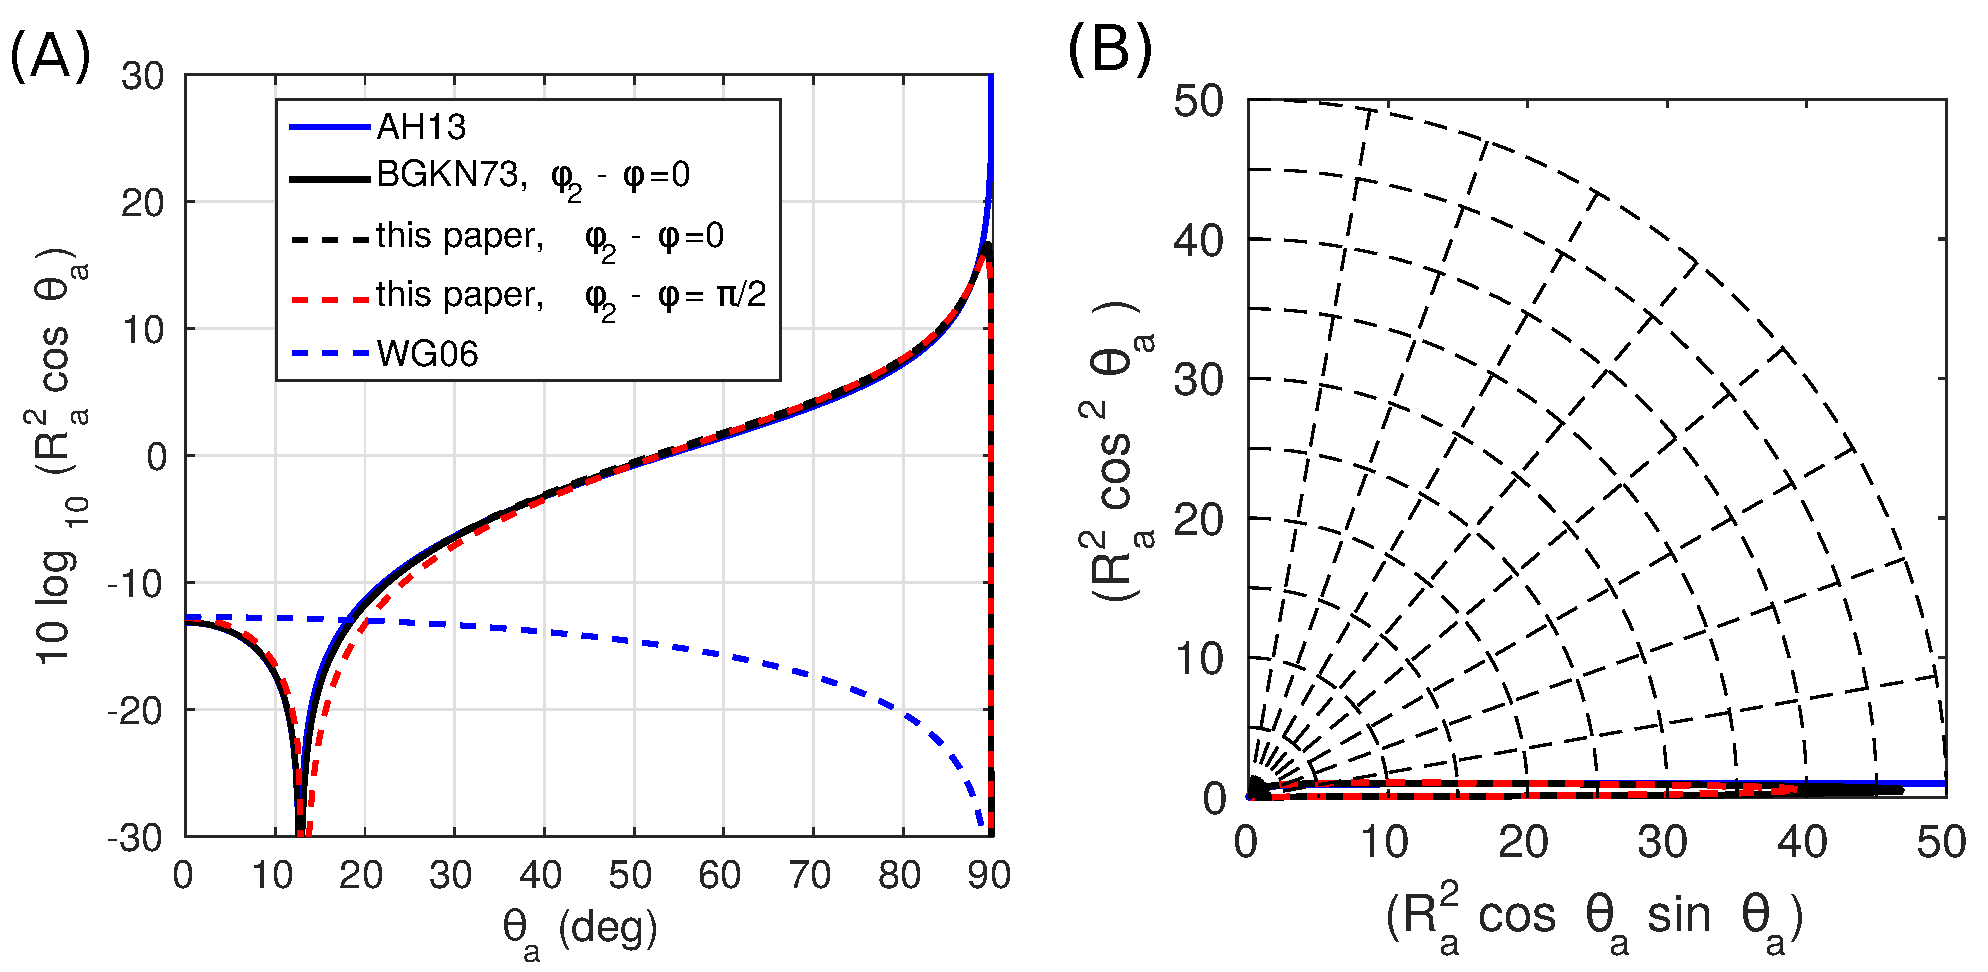
\includegraphics[width=0.8\linewidth]{FIGURES/radiation_deep.pdf}
\caption{Radiation patterns for an ocean wave period of 10~s, given by the different theories without ocean bottom, in cartesian (A), and polar (B) representation, as a function of the acoustic propagation elevation angle $\theta_a$ (measured from the vertical). Note that when the radiated power is considered, these patterns must be multiplied by $\sin \theta_a$ before integration over $\theta_a$. Reproduced from De Carlo et al. (2020). %, as given by eq. (\ref{eq:Power_thetaa}).
  }
\label{fig:rad_deep}
\end{figure}
%%%%%%%%%%%%%%%%%%%%%%%%%%

For a quantitatively correct solution we have to keep all the terms in the equation, including the feedback of the atmospheric pressure on the ocean.
For now, please go to chapter 3 of \cite{DeCarlo2020}. You may find more details here in the next version. In particular I may be brave enough to give you the microbarom source for a 2-layer or $n$-layer atmosphere to show how wave guides can be introduced in the theory without ad hoc handwaving. 




%\cleardoublepage
% \chapter{Generation of waves by the wind}\label{ch_Satm}
% \input{ch_Satm_en}
%\cleardoublepage
%\chapter{Wave breaking and dissipation}\label{ch_sds}
%\input{ch_sds_en}
%\cleardoublepage
%\chapter{Waves in non-homogeneous media}\label{ch_nonhom}
%\input{ch_nonhom}
%\cleardoublepage
%\chapter{Wave-current interactions in three dimensions}\label{ch_vaguescourant3D}
%\input{ch_3Dcur}
%\cleardoublepage

\appendix
\chapter{Some useful tables}
 %%%%%%%%%%%%%%%%%%%%%%%%%%%%%%%%%%%%%%%%%%
\begin{table}
  \centering
  \begin{tabular}{cccccc}
\hline
    $Y=X\tanh(X)$ & $X$     & $Y=X\tanh(X)$ & $X$   & $Y=X\tanh(X)$ & $X$\\
 \hline
       0.05    &     0.2255   &     1.30 & 1.4511 &     2.55  &      2.5795   \\
       0.10    &     0.3216   &     1.35 & 1.4934 &     2.60  &      2.6273   \\
       0.15    &     0.3973   &     1.40 & 1.5360 &     2.65  &      2.6753   \\
       0.20    &     0.4627   &     1.45 & 1.5788 &     2.70  &      2.7234   \\
       0.25    &     0.5218   &     1.50 & 1.6218 &     2.75  &      2.7716   \\
       0.30    &     0.5767   &     1.55 & 1.6651 &     2.80  &      2.8200   \\
       0.35    &     0.6284   &     1.60 & 1.7085 &     2.85  &      2.8684   \\
       0.40    &     0.6778   &     1.65 & 1.7523 &     2.90  &      2.9170   \\
       0.45    &     0.7255   &     1.70 & 1.7962 &     2.95  &      2.9657   \\
       0.50    &     0.7717   &     1.75 & 1.8405 &     3.00  &      3.0145   \\
       0.55    &     0.8168   &     1.80 & 1.8850 &     3.05  &      3.0634   \\
       0.60    &     0.8611   &     1.85 & 1.9297 &     3.10  &      3.1123   \\
       0.65    &     0.9046   &     1.90 & 1.9747 &     3.15  &      3.1613   \\
       0.70    &     0.9476   &     1.95 & 2.0199 &     3.20  &      3.2104   \\
       0.75    &     0.9902   &     2.00 & 2.0653 &     3.25  &      3.2596   \\
       0.80    &     1.0324   &     2.05 & 2.1110 &     3.30  &      3.3088   \\
       0.85    &     1.0744   &     2.10 & 2.1570 &     3.35  &      3.3581   \\
       0.90    &     1.1163   &     2.15 & 2.2031 &     3.40  &      3.4075   \\
       0.95    &     1.1580   &     2.20 & 2.2495 &     3.45  &      3.4569   \\
       1.00    &     1.1997   &     2.25 & 2.2961 &     3.50  &      3.5063   \\
       1.05    &     1.2414   &     2.30 & 2.3428 &   &     \\
       1.10    &     1.2831   &     2.35 & 2.3898 &   &     \\
       1.15    &     1.3249   &     2.40 & 2.4370 &   &     \\
       1.20    &     1.3668   &     2.45 & 2.4843 &   &     \\
       1.25    &     1.4088   &     2.50 & 2.5318 &   &     \\
    \hline                  
\hline
\end{tabular}
  \caption{Table of the inverse function of $X \tanh X$. Defining $Y=\sigma^2 D/g$ it gives $k=X/D$, 
which allows to invert the dispersion relation in the absence of current. 
For $Y< 0.05$ one should use $X=\sqrt{Y}$, and for $Y >3.5$ one should use $X=Y$.}\label{table_tracks}
\end{table}
%%%%%%%%%%%%%%%%%%%%%%%%%%%%%%%%%%%%

%%%%%%%%%%%%%%%%%%%%%%%%%%%%%%%%%%%%%%%%%%%%%%%%%%%%%%%%%%%%%%%%%%%%%%%%%%%%
\begin{figure}
\centerline{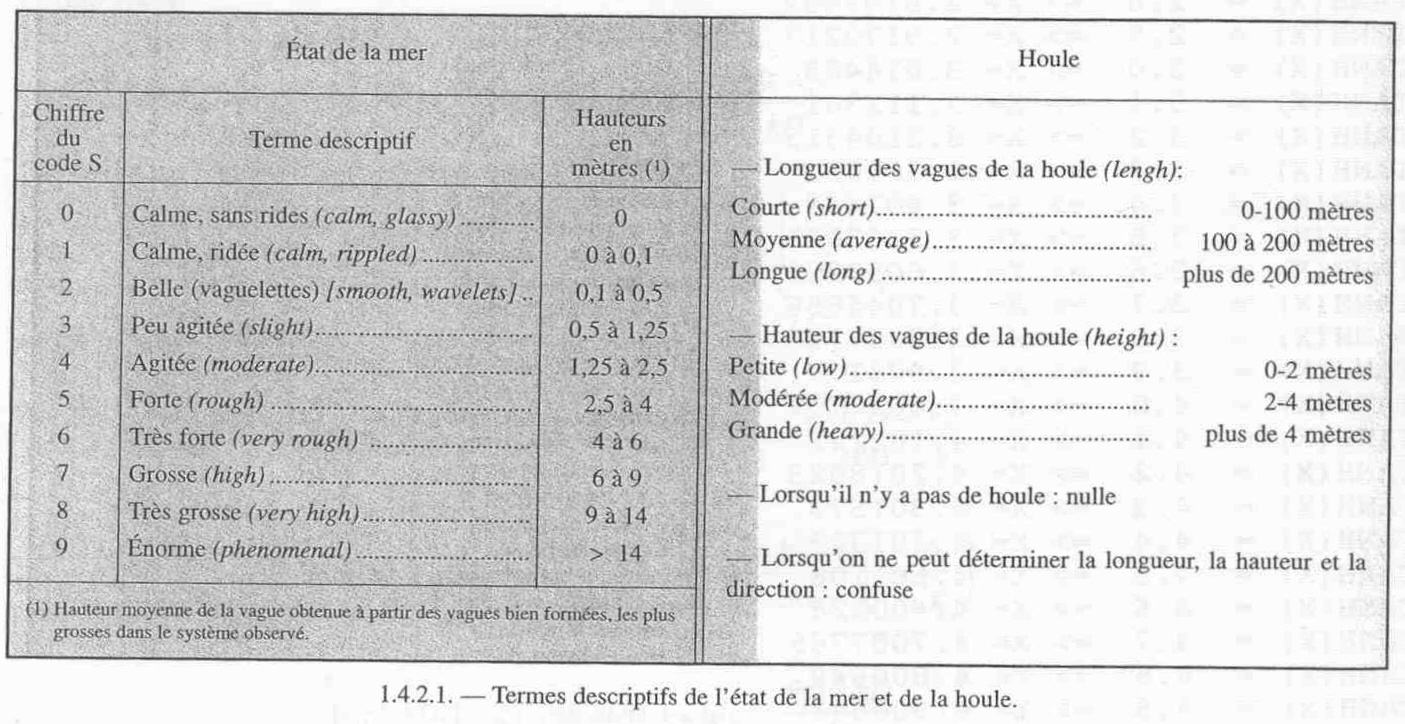
\includegraphics[width=\textwidth]{FIGURES/Table_Beaufort.jpg}}
%\vspace{3.64in}
\caption{The Beaufort scale for sea states \label{table_beaufort}}
\end{figure}
%%%%%%%%%%%%%%%%%%%%%%%%%%%%%%%%%%%%%%%%%%%%%%%%%%%%%%%%%%%%%%%%%%%%%%%%%%%%


%\bibliographystyle{ametsocjmk_nourl}   % si on n'utilise pas  hyperref
\bibliographystyle{ametsocjmk_en}         % avec  hyperref
\bibliography{wave}  % see main.bib; used BibTeX to generate main.bbl




\end{document}        % That's All, Folks!
